\documentclass[a4paper,12pt]{article}

\usepackage{latexsym}
\usepackage[utf8]{inputenc}
\usepackage{graphicx}

\author{Krzysztof~Palka and Dominik~Odrowski}

\title{\textsc{Exercise} 421 \\ Examination of light polarization by reflection phenomena} 

\begin{document}

\maketitle

\begin{abstract}
    This report present the measurement of Brewster's angle for a given material. It shows relation of level of ray polarization depending on incident angle of unpolarized light.    
\end{abstract}

\section{Introduction}
    The aim of this exercise was determining of Brewster's angle for given material and, depending on obtained results, calculation of index of reflection. 


\section{Theory and measurement}
    The light polarized randomly (or unpolarized) is characterized by electric filed at any given point perpendicular to the direction of travel of the waves but changes directions randomly. We can treat unpolarized light as combination of two perpendicular components (polarization S and P) which oscillate perpendicular to component of the electric field (Fig. \ref{fig:sp}\footnote{\cite{HRW}, p. 901}).


\begin{figure}[ht]
    \begin{center}
        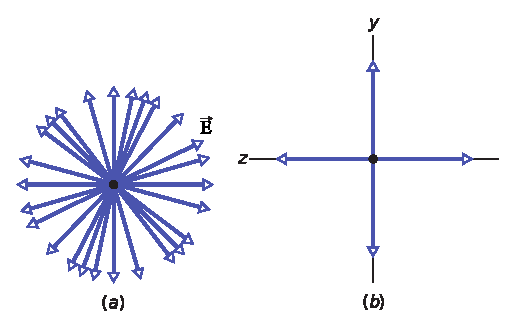
\includegraphics[width=0.65\textwidth]{simplified_polarization}
        \caption{polarization (a) could be simplified as (b)}
        \label{fig:sp}
    \end{center}
\end{figure}
\begin{figure}[ht]
\begin{center}
    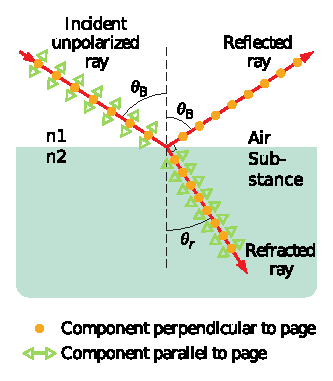
\includegraphics[width=0.35\textwidth]{brewster}
    \caption{temp description}
    \label{fig:brewang}
\end{center}
\end{figure}
Reflected ray is at least partially polarized. When ray incident on dielectric surface with angle $\theta_B$ (Fig. \ref{fig:brewang}\footnote{Ibid., p. 912}), that:
\begin{equation}
    \tan \theta_B = n \label{eq:brew_ang}
\end{equation}
where $n$ is the index of reflection of dielectric, then $\theta_B$ is called Brewster's angle and reflected ray is linearly polarized (electric field vectors on Fig. \ref{fig:brewang} oscillate perpendicular to the page). Incident rays oscillate in perpendicular and parallel directions, so they are unpolarized. Reflected ray behave in similar way, but magnitudes of particular components of electric field oscillations are unequal and that ray is called partially polarized. If incident angle is not equal Brewster's angle, then Reflected ray is also called partially polarized, and level of polarization $K$ can be obtained form equation \ref{eq:K}
\begin{equation}
    K = \frac{I_S-I_P}{I_S+I_P} \label{eq:K}
\end{equation}
Where $I_S$ and $I_S$ are intensities of lights with polarization S and P, according to figure \ref{fig:brewang} respectively perpendicular and parallel to plane determined by diagram.
\begin{figure}[ht]
\begin{center}
    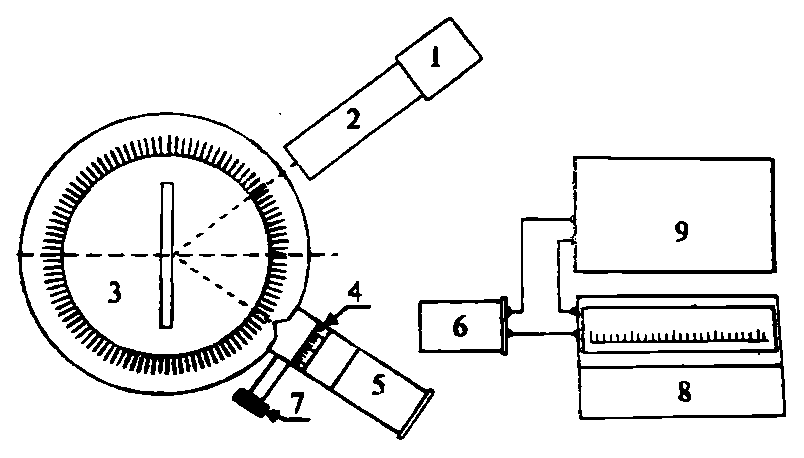
\includegraphics[width=0.65\textwidth]{goniometer}
    \caption{Diagram of the experimental set-up. It consists of swivel table (3) with angular scale of precision $\Delta\alpha = \pm 1^\circ$ and 2 arms. illumination (1) with collimator (2) is placed on fixed arm, analyser (4) and telescope on which could be placed eyepiece (5) or photodetector (6) are mounted on movable arm. Electric circuit consists of photoresistor which is used as photodetector (6), power supply unit (9) and microamperemeter (8)}
    \label{fig:goniometer}
\end{center}
\end{figure}



\begin{thebibliography}{2}
    \bibitem[HRW]{HRW}Fundamentals of physics (2011) [ebook]. David Halliday, Robert Resnick, Jearl Walker. 9th ed. ISBN 978-0-470-46908-8
\end{thebibliography}

\end{document}

